\section{Generaci\'on de tablas JSON y consultas Spark SQL}

\subsection{ETL y tablas generadas}

El ETL lee el CSV desde HDFS o disco local, limpia columnas decimales, castea los campos temporales y genera dos tablas JSON:

\begin{itemize}
    \item \texttt{contribuyentes.json}: dimension de contribuyentes con \texttt{COD\_CONTRIBUYENTE} y \texttt{NOM\_CONTRIBUYENTE}. Se conserva el nombre mas reciente por contribuyente.
    \item \texttt{emisiones.json}: tabla de hechos con granularidad \texttt{(COD\_PREDIO, COD\_CONTRIBUYENTE, PERIODO)}. Esta tabla contiene los montos, descuentos, porcentaje de condominio y ubigeo.
\end{itemize}

La corrida local verifico 222\,874 filas crudas, 47\,175 contribuyentes y 222\,873 emisiones despues de eliminar un duplicado exacto sobre la clave natural de hechos.

\begin{figure}[H]
    \centering
    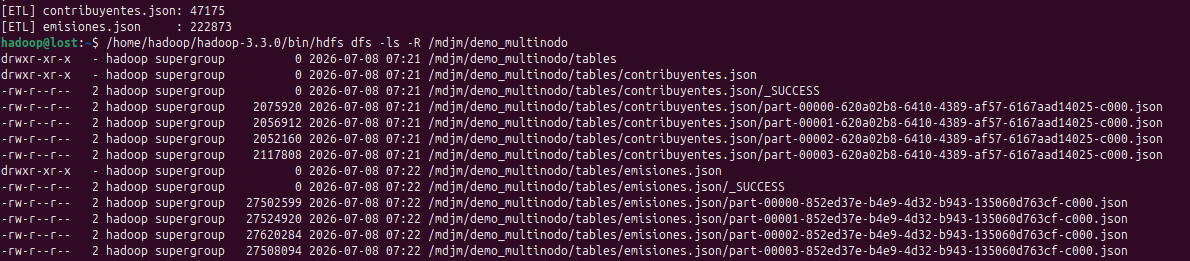
\includegraphics[width=\textwidth]{ImgMultiNodo/json_Contribuyente_emisiones.png}
    \caption{Salidas HDFS generadas por el ETL en \texttt{contribuyentes.json} y \texttt{emisiones.json}.}
    \label{fig:hdfs-tables}
\end{figure}

\subsection{Preguntas respondidas y relacion con el codigo}

La Tabla~\ref{tab:preguntas-consultas} resume, para cada grupo de pregunta solicitado, la consulta analitica que responde, las columnas o caracteristicas empleadas, la solucion implementada, la interpretacion de los resultados y el archivo Scala asociado.

%\begin{longtable}{p{0.12\textwidth}p{0.22\textwidth}p{0.26\textwidth}p{0.25\textwidth}}
\setlength{\emergencystretch}{3em}
\begin{longtable}{
  p{0.12\textwidth}
  p{0.22\textwidth}
  p{0.26\textwidth}
  p{\dimexpr0.40\textwidth-8\tabcolsep\relax}
}
\caption{Preguntas del dataset, solucion aplicada e interpretacion.}

\label{tab:preguntas-consultas}\\

\toprule

\textbf{Item} & \textbf{Pregunta que responde} & \textbf{Columnas/\newline caracteristicas usadas} & \textbf{Solucion e \newline interpretacion} \\

\midrule

\endfirsthead

\toprule

\textbf{Item} & \textbf{Pregunta que responde} & \textbf{Columnas/\newline caracteristicas usadas} & \textbf{Solucion e \newline interpretacion} \\

\midrule

\endhead

ETL y tablas JSON &

¿Como separar el dataset original en estructuras reutilizables sin depender de PostgreSQL? &

\texttt{COD\_CONTRIBUYENTE}, \texttt{NOM\_CONTRIBUYENTE}, \texttt{COD\_PREDIO}, \texttt{PERIODO}, montos, descuentos y \texttt{UBIGEO}. &

Se generan \texttt{contribuyentes.json} y \texttt{emisiones.json}. La primera funciona como dimension y la segunda como tabla de hechos a nivel predio-contribuyente-periodo. Codigo: \texttt{ETL.scala}. \\

\midrule

SQL 1: \texttt{groupBy} + funciones &

¿Cuanto se emitio en total y en promedio por concepto municipal durante cada periodo? &

\texttt{PERIODO}, \texttt{MONTO\_PARQUE\_JARDIN}, \texttt{MONTO\_SERENAZGO}, \texttt{MONTO\_RESIDUO\_SOLIDO}, \texttt{MONTO\_BARRIDO\_CALLE}. &

Se agrupa por periodo y se aplican \texttt{sum}, \texttt{avg}, \texttt{count} y \texttt{round}. Permite comparar la evolucion anual de la emision por concepto. Codigo: \texttt{SqlQueries.query1GroupByPeriodo}. \\

\midrule

SQL 2: vista temporal + \texttt{ORDER BY} &

¿Cuales son los predios exclusivos con mayor monto total neto en 2025? &

\texttt{COD\_PREDIO}, \texttt{COD\_CONTRIBUYENTE}, \texttt{PERIODO}, \texttt{PORCENTAJE\_CONDOMINIO}, montos y descuentos. &

Se crea una vista temporal y se filtra 2025 con condominio 100. Luego se calcula monto neto y se ordena de mayor a menor. Codigo: \texttt{SqlQueries.query2TopPrediosTempView}. \\

\midrule

Regresion MLP &

¿Se puede estimar el monto de serenazgo a partir de variables monetarias y del periodo? &

\texttt{MONTO\_SERENAZGO} como etiqueta; \texttt{PERIODO}, \texttt{PORCENTAJE\_CONDOMINIO}, montos y descuentos como features. &

Se implementa un MLP de regresion con salida lineal y perdida MSE. El menor RMSE frente a SVR indica mejor ajuste global para esta tarea. Codigo: \texttt{MLPRegressor.scala}. \\

\midrule

Regresion SVR &

?Como se comporta una regresion basada en SVM para estimar serenazgo? &

Mismas variables de regresion que MLP para mantener comparabilidad. &

Se implementa SVR lineal con perdida epsilon-insensitiva. Tiene resultados positivos, pero mayor RMSE que MLP. Codigo: \texttt{SVRegressor.scala}. \\

\midrule

Clasificacion Random Forest &

¿Se puede clasificar un predio como exclusivo o compartido usando variables decimales sin fuga de datos? &

\texttt{TIPO\_PREDIO} como etiqueta derivada; se excluye \texttt{PORCENTAJE\_CONDOMINIO} de las features para evitar fuga. &

Random Forest logra el mejor F1-score. Su interpretacion es que los arboles capturan mejor reglas por umbral y relaciones no lineales. Codigo: \texttt{RFAndMLPClassification.scala}. \\

\midrule

Clasificacion MLP &

¿Que desempeno tiene una red neuronal para clasificar tipo de predio frente a Random Forest? &

Mismas variables de clasificacion que Random Forest. &

MLPClassifier funciona, pero obtiene menor F1-score que Random Forest, por lo que requiere mayor ajuste. Codigo: \texttt{RFAndMLPClassification.scala}. \\

\bottomrule

\end{longtable}

\subsection{Consulta 1: recaudacion por periodo}

\textbf{Pregunta de an\'alisis:} \textquestiondown Cu\'anto se emiti\'o en total y en promedio por concepto municipal durante cada periodo?

La primera consulta utiliza la API DataFrame de Spark con \texttt{groupBy("PERIODO")} y funciones de \texttt{org.apache.spark.sql.functions}: \texttt{sum}, \texttt{avg}, \texttt{round} y \texttt{count}. El resultado permite comparar la evolucion anual de los conceptos de parques y jardines, serenazgo, residuos solidos y barrido de calles.

\begin{table}[H]
    \centering
    \caption{Resultado de la consulta 1: totales y promedios por periodo.}
    \label{tab:query1}
    \resizebox{\textwidth}{!}{%
    \begin{tabular}{rrrrrrrrr}
        \toprule
        \textbf{Periodo} & \textbf{Total parques} & \textbf{Prom. parques} & \textbf{Total serenazgo} & \textbf{Prom. serenazgo} & \textbf{Total residuos} & \textbf{Prom. residuos} & \textbf{Total barrido} & \textbf{Emisiones} \\
        \midrule
        2023 & 11\,744\,689.56 & 168.07 & 24\,439\,219.92 & 349.73 & 9\,683\,019.72 & 138.57 & 2\,643\,129.06 & 69\,880 \\
        2024 & 12\,587\,472.36 & 170.15 & 26\,232\,272.82 & 354.59 & 8\,767\,155.37 & 118.51 & 2\,820\,661.03 & 73\,980 \\
        2025 & 11\,919\,521.07 & 150.86 & 27\,835\,182.83 & 352.29 & 9\,816\,547.57 & 124.24 & 3\,314\,446.63 & 79\,013 \\
        \bottomrule
    \end{tabular}}
\end{table}


\subsection{Consulta 2: top de predios exclusivos 2025}

\textbf{Pregunta de an\'alisis:} \textquestiondown Cu\'ales son los predios de propiedad exclusiva con mayor monto total neto en 2025?

La segunda consulta registra \texttt{emisiones} como vista temporal y ejecuta SQL con filtros \texttt{WHERE PERIODO = 2025} y \texttt{PORCENTAJE\_CONDOMINIO = 100}, calculando el monto total neto y ordenando de forma descendente con \texttt{ORDER BY}. La salida final se limita a los 20 predios principales.

\begin{table}[H]
    \centering
    \caption{Primeros 10 registros del top 20 de predios exclusivos 2025 por monto total neto.}
    \label{tab:query2}
    \resizebox{\textwidth}{!}{%
    \begin{tabular}{llrr}
        \toprule
        \textbf{COD\_PREDIO} & \textbf{COD\_CONTRIBUYENTE} & \textbf{Periodo} & \textbf{Monto neto} \\
        \midrule
        6ffc4409...fd253b6 & 38548de4...f0788ef56 & 2025 & 284\,967.96 \\
        6caa5d8c...e4b6ca27 & c55edd28...8d6d48b72 & 2025 & 238\,877.52 \\
        651ead64...87fc39e1 & 38548de4...f0788ef56 & 2025 & 203\,219.88 \\
        48f6cd74...7967f794 & 39ed9d90...665df386 & 2025 & 193\,386.84 \\
        a95619fe...e16a14092 & 39ed9d90...665df386 & 2025 & 190\,837.20 \\
        08bd0c59...51e9d156 & 4539797a...4397e739 & 2025 & 187\,427.40 \\
        ba03f0a6...ebda7ec0 & 38548de4...f0788ef56 & 2025 & 178\,622.28 \\
        2c210356...c38f58fb & 549998ab...3c379ed & 2025 & 175\,102.68 \\
        1d97b755...abb9073e & 55351ada...0abb9073e & 2025 & 148\,005.60 \\
        3db57089...a933474 & d5c17c98...ceb885ed & 2025 & 144\,528.84 \\
        \bottomrule
    \end{tabular}}
\end{table}


\begin{figure}[H]
    \centering
    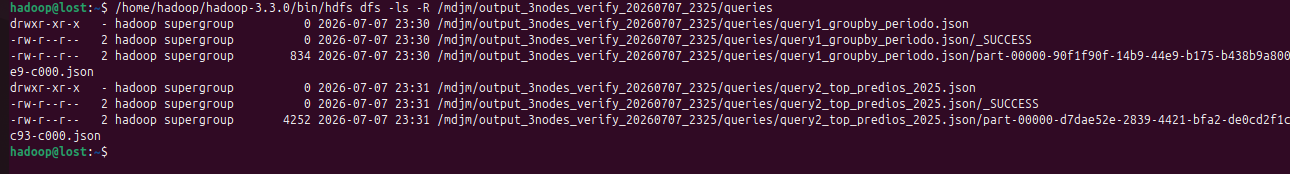
\includegraphics[width=\textwidth]{ImgMultiNodo/json_query_1_2.png}
    \caption{Directorios HDFS generados para las dos consultas Spark SQL.}
    \label{fig:hdfs-queries}
\end{figure}

\begin{figure}[H]
    \centering
    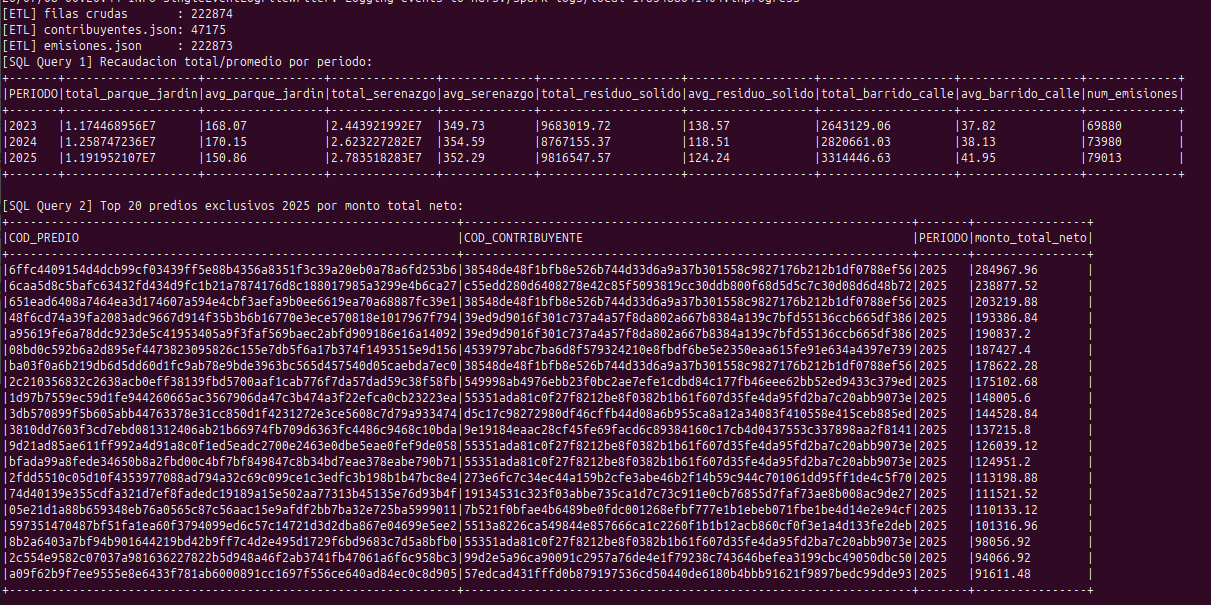
\includegraphics[width=\textwidth]{ImgNod1/ETL_SQL.png}
    \caption{Ejecucion mononodo: conteos ETL y resultados de las dos consultas en terminal.}
    \label{fig:local-etl-sql}
\end{figure}
